\section{Common-witness geometry and interval tools}
\label{sec:geometry}

Using the notation of Definition~\ref{def:normalized-queries},
we prove the structural facts shared by both algorithms.
Algorithm~\ref{alg:hull-data} records their common preprocessing.
Flat states admit a common majority witness, each normalized query
has at most two adjacent hull supports, and each hypothesis has
one circular positive interval. The interval tools below cover
these patterns and recover their endpoints without adding queries.

\begin{symboltable}
$p,\ x_h,\ u_i$ & Strict common witness, translated hypothesis vector $h-p$, and normalized vector for supplied line $\ell_i$.\\
$C_i,\ R_h$ & Original-plane cap opposite $p$ for query $i$, and the dual set of normalized queries positive on $h$.\\
$K,\ V$ & Convex hull of the normalized query vectors together with $0$, and its nonzero vertices in cyclic order.\\
$J_i,\ \alpha_{iv}$ & At most two adjacent support vertices for $u_i$ and their nonnegative coefficients, whose sum is at most one.\\
$\sigma(h),\ \Pi$ & Hull-test bit pattern of $h$ and the partition into equal-pattern classes.\\
$A_0,\ b(S)$ & All-zero pattern class (empty if absent) and, with priors, the mass outside that class.\\
$g_A$ & First positive test position for a nonzero pattern class $A$ in a discovery schedule.\\
\end{symboltable}

\subsection{A common majority witness}

\begin{lemma}[Common witness]\label{lem:helly}
In either kind of flat state, a point $p$ strictly inside every
majority half-plane can be computed in polynomial time.
\end{lemma}
\begin{proof}
Use the measure defining flatness, either cardinality or probability.
The union of any three minority caps has measure less than
$3\delta$ times the measure of $S$, and therefore omits a hypothesis.
That hypothesis belongs strictly to all three majority half-planes,
because no hypothesis lies on a query line. The same argument covers
subfamilies of fewer than three lines. Thus every subfamily of at
most three majority half-planes has nonempty intersection.
Theorem~\ref{thm:helly} implies
that the whole family has nonempty intersection.

To obtain a strict rational witness, orient each majority inequality
as $a_i\cdot p-b_i>0$ and maximize $t$ subject to
$a_i\cdot p-b_i\ge t$ for every $i$ and $0\le t\le1$.
The open intersection supplies a feasible positive $t$.
This is a \emph{linear program}: its objective and constraints
are linear in the unknown coordinates of $p$ and the margin $t$.
Rational linear programming therefore returns a strict witness
with polynomial encoding length~\cite{khachiyan1979}.
\end{proof}

\subsection{Adjacent supports and circular patterns}

\begin{lemma}[Hull support and pattern structure]\label{lem:hull-structure}
The support blocks of Definition~\ref{def:normalized-queries} can
be chosen with at most two real hull vertices, adjacent when there
are two. For every query,
\begin{equation}\label{eq:hull-cap-cover}
 C_i\cap S\ \subseteq\ \bigcup_{v\in J_i}(C_v\cap S).
\end{equation}
Negative support bits force the query's witness-side answer.
The positive vertices of every hypothesis form a circular interval,
$|A_0|\le1$, and every nonzero pattern class lies in a positive hull cap.
\end{lemma}
\begin{proof}
Extend the ray from $0$ through $u_i$ to its last point $y$ in $K$.
If $y$ lies on an edge with endpoints $v,w$, write
$y=\theta v+(1-\theta)w$ and $u_i=\lambda y$, with
$0<\lambda\le1$. The resulting coefficients are nonnegative and
sum to $\lambda\le1$. Delete origin endpoints and zero coefficients
to obtain $J_i$. A boundary vertex needs only itself.
In dimension at most one, the last ray point is a segment endpoint,
so the same conclusion holds directly.

If every support has $v\cdot x_h\le1$, then
$u_i\cdot x_h=\sum_{v\in J_i}\alpha_{iv}(v\cdot x_h)
\le\sum_v\alpha_{iv}\le1$. This proves
\eqref{eq:hull-cap-cover}. Equality cannot occur at a hypothesis
because it would put it on the original supplied line.
The origin has dot product zero, so its bit is always negative
and it is never queried.

The positive vertices are $V\cap R_h$.
A half-plane selects a consecutive block of a convex polygon's
vertices. Removing the known-negative origin, if it is a vertex,
leaves a circular interval on $V$. Degenerate hulls have at most
two real vertices and satisfy the same assertion.
An all-zero pattern forces every original query to have the
witness's answer; two such hypotheses would contradict separability.
Finally, a nonzero class has some positive vertex $v$, and all
its hypotheses belong to $C_v\cap S$.
\end{proof}

\begin{algorithm}[H]
\caption{\HullData: a flat state's witness, supports, and patterns}
\label{alg:hull-data}
\KwIn{Flat state $S$ and its count or mass measure; supplied lines.}
\KwOut{Strict witness $p$, full hull $K$, real vertices $V$, supports $J_i$, partition $\Pi$.}
Orient every majority inequality as $a_i\cdot p-b_i>0$\;
Maximize $t$ subject to $a_i\cdot p-b_i\ge t$ and $0\le t\le1$;
retain a solution with $t>0$\;
Compute $u_i=-a_{\ell_i}/f_{\ell_i}(p)$ and
$K=\operatorname{conv}(\{0\}\cup\{u_i\})$\;
Keep one supplied representative of each real hull vertex in cyclic order\;
\ForEach{$u_i$}{
Extend its ray from $0$ to the last point $y$ in $K$\;
Express $y$ on its boundary edge and scale the coefficients by
$\|u_i\|/\|y\|$; omit the origin and zero coefficients to form $J_i$\;
}
Compute all bits $\mathbf1[v\cdot(h-p)>1]$ and group equal rows into $\Pi$\;
\KwRet $(p,K,V,(J_i),\Pi)$, retaining the origin's boundary position\;
\end{algorithm}

The ray scaling is obtained from rational coordinates, without a
square-root computation. In dimension at most one use segment
endpoints as supports. Lemmas~\ref{lem:helly} and
\ref{lem:hull-structure} prove feasibility and the support invariant.


Figure~\ref{fig:support-and-interval} separates the two geometric
roles: panel (a) shows how adjacent hull vertices support an original
query vector, while panel (b) records only the cyclic order of the
hull tests seen positively by one hypothesis.

\begin{figure}[tbp]
\centering
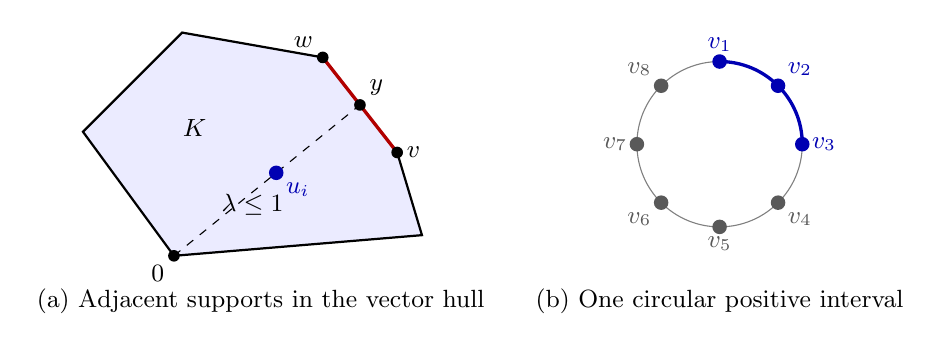
\begin{tikzpicture}[scale=1.05,every node/.style={font=\small}]
  % Query vectors and their adjacent hull supports.
  \fill[blue!8]
    (0,0)--(3,0.25)--(2.7,1.25)--(1.8,2.4)--(0.1,2.7)
    --(-1.1,1.5)--cycle;
  \draw[thick]
    (0,0)--(3,0.25)--(2.7,1.25)--(1.8,2.4)--(0.1,2.7)
    --(-1.1,1.5)--cycle;
  \draw[very thick,red!70!black] (2.7,1.25)--(1.8,2.4);
  \draw[dashed] (0,0)--(2.25,1.825);
  \fill (0,0) circle (2pt) node[below left] {$0$};
  \fill (2.7,1.25) circle (2pt) node[right] {$v$};
  \fill (1.8,2.4) circle (2pt) node[above left] {$w$};
  \fill (2.25,1.825) circle (2pt) node[above right] {$y$};
  \fill[blue!70!black] (1.2375,1.00375) circle (2.5pt)
    node[below right] {$u_i$};
  \node at (0.25,1.55) {$K$};
  \node at (0.95,0.62) {$\lambda\le1$};
  \node[align=center] at (1.05,-0.55)
    {(a) Adjacent supports in the vector hull};

  % A schematic cyclic order; blue vertices form one interval.
  \draw[gray] (6.6,1.35) circle (1);
  \draw[very thick,blue!70!black]
    (6.6,2.35) arc[start angle=90,end angle=0,radius=1];
  \fill[blue!70!black] (6.6,2.35) circle (2.5pt)
    node[above] {$v_1$};
  \fill[blue!70!black] (7.307,2.057) circle (2.5pt)
    node[above right] {$v_2$};
  \fill[blue!70!black] (7.6,1.35) circle (2.5pt)
    node[right] {$v_3$};
  \fill[gray!70!black] (7.307,0.643) circle (2.5pt)
    node[below right] {$v_4$};
  \fill[gray!70!black] (6.6,0.35) circle (2.5pt)
    node[below] {$v_5$};
  \fill[gray!70!black] (5.893,0.643) circle (2.5pt)
    node[below left] {$v_6$};
  \fill[gray!70!black] (5.6,1.35) circle (2.5pt)
    node[left] {$v_7$};
  \fill[gray!70!black] (5.893,2.057) circle (2.5pt)
    node[above left] {$v_8$};
  \node[align=center] at (6.6,-0.55)
    {(b) One circular positive interval};
\end{tikzpicture}
\caption{The first panel depicts normalized query vectors, not
hypotheses: $y$ lies on the edge $vw$ and $u_i=\lambda y$ for
$0<\lambda\le1$. Writing $y=\theta v+(1-\theta)w$ gives
$u_i=\alpha v+\beta w$ with $\alpha+\beta=\lambda\le1$.
Consequently, if both support values on a hypothesis are at most
one, then $u_i\cdot x_h\le1$; equivalently,
$C_i\subseteq C_v\cup C_w$. The second panel shows the cyclic order
only; the positive hull tests of a fixed hypothesis form one
interval in that order.}
\label{fig:support-and-interval}
\end{figure}

\subsection{Interval hitting and discovery length}

\begin{lemma}[Minimum interval cover]\label{lem:minimum-interval-cover}
A minimum-cardinality hitting set for ordinary or circular intervals
on a finite candidate order is computable in polynomial time.
An empty demand is infeasible; an empty family needs no candidates.
\end{lemma}
\begin{proof}
For ordinary intervals, choose the right endpoint $q$ of an
earliest-ending interval $I$. Any cover has a point $u\in I$.
Replacing $u$ by $q$ loses no demand containing $u$: its right
endpoint is at least $q$ and its left endpoint is at most $u\le q$.
Thus an optimal cover can choose $q$. Delete the intervals hit
there and repeat, proving the endpoint greedy rule is exact.

For circular intervals, choose a nonempty demand and enumerate
a forced candidate $v$ in it. Delete demands hit by $v$ and cut
the cycle there. All remaining demands are ordinary intervals,
so use the preceding rule and add $v$. Some forced choice belongs
to an optimal circular cover; take the smallest resulting solution.
\end{proof}

\begin{lemma}[Greedy cover length with adjacent-run credit]
\label{lem:greedy-cover-length}
Let a nonempty family of positively weighted interval demands
be covered by a candidate set $P$ of size $k$. Let $c(P)$ be the
number of runs of consecutive candidates in $P$, measured in the
entire candidate order. Maximum-remaining-weight greedy finishes
within $k+c(P)-1$ choices, for every tie rule.
In particular, a minimum cover of size $k$ gives the usual bound
$2k-1$. For circular intervals the corresponding bound is $2k$.
\end{lemma}
\noindent
The extra term is the number of runs beyond the first. A scattered
cover may force greedy to spend choices repairing several gaps,
whereas a cover arranged in a few contiguous blocks has fewer such
gaps to repair.
\begin{proof}
Induct on $k$. When $k=1$, its sole candidate hits every demand,
and any greedy maximum does so as well.

Let $v$ be the first greedy choice. If it lies at or outside an
extreme of $P$, let $u$ be the nearest extreme cover point.
For example, if $v<\min P=u$, every demand containing $v$ must also
meet $P$, and hence must contain $u$. Thus the demands hit by $v$
are a subset of those hit by $u$. Greedy maximality gives the reverse
inequality on their total weights, so the two candidates hit the
same positive-weight demands.
Thus $P\setminus\{u\}$ covers the remainder, and removing an
extreme does not increase its run count. Induction plus the first
query gives at most $k+c(P)-1$ choices.

Otherwise $v$ lies strictly between the extremes of $P$.
The unhit intervals lie entirely on one side of $v$.
The parts $P_-,P_+$ strictly to its left and right cover these
two families, and
\[
 |P_-|+c(P_-)+|P_+|+c(P_+)\le k+c(P).
\]
If $v\notin P$, cutting in its gap leaves the total run count
unchanged. If $v\in P$, removing it reduces size by one and can
increase total run count by at most one, which proves the displayed
inequality in either case. Greedy may interleave the two sides, but
a choice on one side covers no interval on the other; hence the
choices restricted to either side are still a greedy sequence for
that side. If both families are nonempty,
induction plus the first query gives
\[
 1+\bigl(|P_-|+c(P_-)-1\bigr)
   +\bigl(|P_+|+c(P_+)-1\bigr)\le k+c(P)-1.
\]
If only one is nonempty, the other cover part still has size plus
run count at least two, so the same bound holds. If neither
remains, one query suffices.
Finally $c(P)\le k$, giving $2k-1$ without adjacency information.

For circular intervals, make the first greedy choice and cut the
cycle there. Every unhit interval becomes an ordinary interval.
The original $k$ cover candidates still cover these demands,
so at most $2k-1$ further choices are needed.
\end{proof}

\subsection{Recovering the interval endpoints}
\label{sec:endpoint-geometry}

After discovery, one positive hull vertex $v$ is known.
First inspect its cached neighbor answers. If a neighbor is known
to be negative, cut at that vertex and orient the order so that
$v$ is first. The positive interval starts at $v$, so only its
other endpoint needs a search. If both neighbors are negative,
the pattern consists of $v$ alone and no endpoint query is needed.

Otherwise use a geometric cut. If the origin lies on the hull
boundary, cut at its free negative
marker. If it is interior, the ray from $v$ through $0$ meets
an opposite hull edge with consecutive endpoints $a,b$.
The origin is a convex combination of $v,a,b$, with positive
coefficient on $v$. Thus $a,b$ cannot both be positive: if all
three dot products with $x_h$ exceeded one, their convex
combination would also exceed one, contradicting $0\cdot x_h=0$.
Cut the cyclic order between $a$ and $b$. A circular positive
interval could wrap around this cut only if both endpoints
were positive, which was just excluded. If the ray meets a
vertex, that vertex is necessarily negative and is itself a
free cut point.

No anchor query is made. The positive vertices now form an
ordinary interval containing $v$. To its left, querying a vertex asks whether
the left endpoint is at or before that vertex. To its right,
querying a vertex asks whether the right endpoint is at or after it.
Thus supplied hull queries give exactly the ordered comparisons
needed to locate the two endpoints.



When neither endpoint is already fixed, learn the left endpoint,
then the right endpoint conditioned on
the left endpoint and the earlier transcript. For consecutive
possible left endpoints, querying the earlier endpoint separates
them; for consecutive possible right endpoints, querying the later
endpoint separates them. These are real hull vertices, so all
comparisons used by the codes are supplied queries.
The conditional endpoint distributions come from the hypothesis table.

If $K$ has dimension at most one, it has at most two real vertices.
With two real endpoints, one positive endpoint forces the other
negative because $0$ lies between them. With one real vertex,
its positive bit is the complete nonzero pattern.
Thus no further query is needed in either degenerate case.

A positive discovery exit is \emph{pinned} if a neighbor of its
discovered vertex has a cached negative answer. It is
\emph{singly pinned} when exactly one neighbor is known negative,
and \emph{doubly pinned} when both are. Pinning fixes one or both
endpoints, as described above; it introduces no additional query.

\begin{algorithm}[H]
\caption{\EndpointCode: legal full-pattern recovery}
\label{alg:endpoint-code}
\KwIn{A positive hull vertex $v$, compatible patterns, cached answers;
code mode; optionally fixed continuation heights $h_A$.}
\KwOut{A supplied-query decoder whose leaves are full pattern classes.}
\If{the hull has dimension at most one}{\KwRet the already determined nonzero pattern\;}
\eIf{$v$ has a cached negative neighbor}{
  Cut at that neighbor and orient so $v$ is the first positive vertex\;
}{
  Cut at a boundary origin, or at the opposite edge met by the ray $v0$\;
}
List the realized left and right endpoint pairs in the cut order\;
\eIf{no continuation heights are supplied}{
  Search each unfixed endpoint using Algorithm~\ref{alg:alphabetic-code};
  condition the second search on the first answer\;
}{
  \ForEach{endpoint rectangle $R$, in increasing size}{
    \eIf{$R$ has a single realized class $A$}{$E(R)\gets h_A$\;}{
      $E(R)\gets\min_\ell(1+\max\{E(R\cap\ell^-),E(R\cap\ell^+)\})$,
      over proper supplied endpoint thresholds\;
    }
  }
  Reconstruct the minimizing rectangle splits and attach the fixed child codes\;
}
\KwRet the decoder; skip fixed endpoints and cached thresholds\;
\end{algorithm}

Section~\ref{sec:endpoint-geometry} proves the cut is legal without an
anchor query. With continuation heights this is the complete-exit
optimization of Section~\ref{sec:polynomial-slots}; its $O(M^4)$
rectangles and $O(M)$ thresholds give polynomial running time.

